\documentclass[t,usenames,dvipsnames]{beamer}
\usetheme{Copenhagen}
\setbeamertemplate{headline}{} % remove toc from headers
\beamertemplatenavigationsymbolsempty

\usepackage{amsmath, tikz, xcolor, bm, pgfplots, array}
\pgfplotsset{compat = newest}
\tikzset{>=stealth}
\usetikzlibrary{arrows, calc, decorations.pathreplacing, patterns}

\title{Angle Sum and Difference Identities}
\author{}
\date{}

\AtBeginSection[]
{
  \begin{frame}
    \frametitle{Objectives}
    \tableofcontents[currentsection]
  \end{frame}
}

\begin{document}

\begin{frame}
    \titlepage
\end{frame}

\section{Solve problems using angle sum and difference identities}

\begin{frame}{$\cos(A-B)$}
\begin{tabular}{ll}
    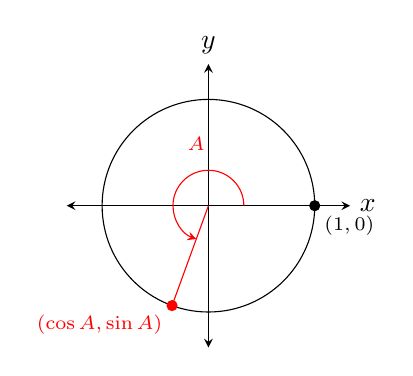
\begin{tikzpicture}[scale=0.9]
    \draw [<->] (-2,0) -- (2,0) node [right] {$x$};
    \draw [<->] (0,-2) -- (0,2) node [above] {$y$};
    \draw (0,0) circle (1.5cm);
    \draw [fill] (1.5,0) circle (2pt) node [below right] {\scriptsize $(1,0)$};
    \draw [fill,red] (250:1.5) circle (2pt) node [below left] {\scriptsize $(\cos A, \sin A)$};
    \draw [red] (0,0) -- (250:1.5);
    \draw [red, ->] (0.5,0) arc (0:250:0.5) node [above, yshift=1cm] {\scriptsize $A$};
    \end{tikzpicture}
    &
    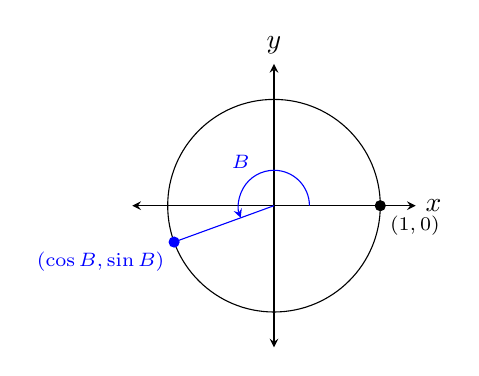
\begin{tikzpicture}[scale=0.9]
    \draw [<->] (-2,0) -- (2,0) node [right] {$x$};
    \draw [<->] (0,-2) -- (0,2) node [above] {$y$};
    \draw (0,0) circle (1.5cm);
    \draw [fill] (1.5,0) circle (2pt) node [below right] {\scriptsize $(1,0)$};
    \draw [fill,blue] (200:1.5) circle (2pt) node [below left] {\scriptsize $(\cos B, \sin B)$};
    \draw [blue] (0,0) -- (200:1.5);
    \draw [blue, ->] (0.5,0) arc (0:200:0.5) node [above, yshift=0.5cm] {\scriptsize $B$};
    \end{tikzpicture}
\end{tabular}
\end{frame}

\begin{frame}{$\cos(A-B)$}
\begin{center}
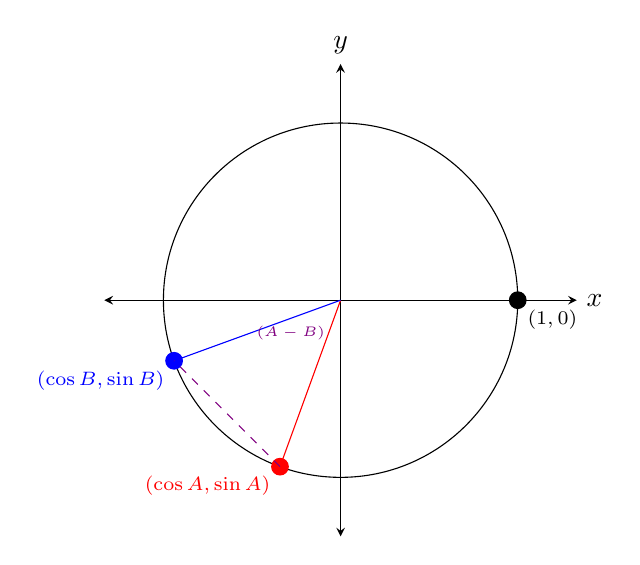
\begin{tikzpicture}[scale=1.5]
    \draw [<->] (-2,0) -- (2,0) node [right] {$x$};
    \draw [<->] (0,-2) -- (0,2) node [above] {$y$};
    \draw (0,0) circle (1.5cm);
    \draw [fill] (1.5,0) circle (2pt) node [below right] {\scriptsize $(1,0)$};
    \draw [fill,red] (250:1.5) circle (2pt) node [below left] {\scriptsize $(\cos A, \sin A)$};
    \draw [fill,blue] (200:1.5) circle (2pt) node [below left] {\scriptsize $(\cos B, \sin B)$};
    \draw [red] (0,0) -- (250:1.5);
    \draw [blue] (0,0) -- (200:1.5);
    \node at (-0.25,0) [below left, yshift=-0.2cm, xshift=0.3cm] {\color{violet} \tiny $(A-B)$};
    \draw [dashed, violet] (250:1.5) -- (200:1.5);
    \end{tikzpicture}
\end{center}
\end{frame}

\begin{frame}{$\cos(A-B)$}
\begin{center}
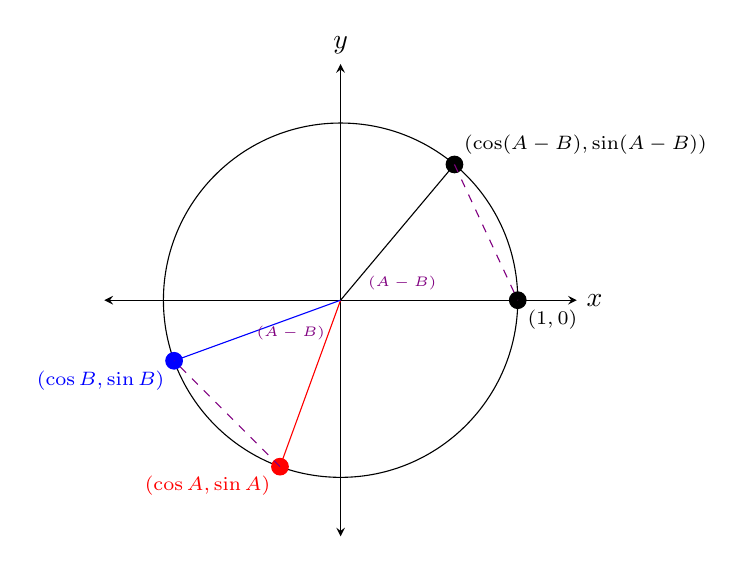
\begin{tikzpicture}[scale=1.5]
    \draw [<->] (-2,0) -- (2,0) node [right] {$x$};
    \draw [<->] (0,-2) -- (0,2) node [above] {$y$};
    \draw (0,0) circle (1.5cm);
    \draw [fill] (1.5,0) circle (2pt) node [below right] {\scriptsize $(1,0)$};
    \draw [fill,red] (250:1.5) circle (2pt) node [below left] {\scriptsize $(\cos A, \sin A)$};
    \draw [fill,blue] (200:1.5) circle (2pt) node [below left] {\scriptsize $(\cos B, \sin B)$};
    \draw [red] (0,0) -- (250:1.5);
    \draw [blue] (0,0) -- (200:1.5);
    \node at (-0.25,0) [below left, yshift=-0.2cm, xshift=0.3cm] {\color{violet} \tiny $(A-B)$};
    \draw [dashed, violet] (250:1.5) -- (200:1.5);
    \draw (0,0) -- (50:1.5) node [above right] {\scriptsize $(\cos(A-B), \sin(A-B))$};
    \draw [fill] (50:1.5) circle (2pt);
    \draw [dashed, violet] (50:1.5) -- (1.5,0);
    \node at (0.15,0) [above right] {\color{violet} \tiny $(A-B)$};
    \end{tikzpicture}
\end{center}
\end{frame}

\begin{frame}{Distance Between $(\cos A, \sin A)$ and $(\cos B, \sin B)$}
    \begin{align*}
        &\sqrt{(\cos A - \cos B)^2 + (\sin A - \sin B)^2} \\[10pt]
        \onslide<2->{&=\sqrt{\cos^2A - 2\cos A \cos B + \cos^2 B + \sin^2A - 2\sin A \sin B + \sin^2 B}} \\[10pt]
        \onslide<3->{&=\sqrt{1 - 2\cos A \cos B - 2\sin A \sin B + 1}} \\[10pt]
        \onslide<4->{&=\sqrt{2-2\cos A \cos B - 2\sin A \sin B}}
    \end{align*}
\end{frame}

\begin{frame}{Distance between $(\cos(A-B), \sin(A-B))$ and $(1,0)$}
    \begin{align*}
    &\sqrt{(\cos(A-B) - 1)^2 + (\sin(A-B) - 0)^2} \\[10pt]
    \onslide<2->{&=\sqrt{\cos^2(A-B) - 2\cos(A-B) + 1 + \sin^2(A-B)}} \\[10pt]
    \onslide<3->{&=\sqrt{1 - 2\cos(A-B) + 1}} \\[10pt]
    \onslide<4->{&=\sqrt{2-2\cos(A-B)}} 
    \end{align*}
\end{frame}

\begin{frame}{Equal distances}
    \begin{align*}
        \sqrt{2-2\cos(A-B)} &= \sqrt{2-2\cos A \cos B - 2\sin A \sin B} \\[10pt]
        \onslide<2->{2-2\cos(A-B) &= 2-2\cos A \cos B - 2\sin A \sin B} \\[10pt]
        \onslide<3->{-2\cos(A-B) &= -2\cos A \cos B - 2\sin A \sin B} \\[10pt]
        \onslide<4->{\cos(A-B) &= \cos A \cos B + \sin A \sin B}
    \end{align*}
\end{frame}

\begin{frame}{Example 1}
    Find the \emph{exact} value of $\cos 15^\circ$.
    \begin{align*}
        \onslide<2->{\cos 15^\circ &= \cos(45^\circ - 30^\circ)} \\[8pt]
        \onslide<3->{&= \cos 45^\circ \cdot \cos 30^\circ + \sin 45^\circ \cdot \sin 30^\circ} \\[8pt]
        \onslide<4->{&= \dfrac{\sqrt{2}}{2} \quad \cdot \quad  \dfrac{\sqrt{3}}{2} \quad + \quad \dfrac{\sqrt{2}}{2} \quad \cdot \quad  \dfrac{1}{2} } \\[8pt]
        \onslide<5->{&=\dfrac{\sqrt{6}}{4} \qquad + \qquad \dfrac{\sqrt{2}}{4}} \\[8pt]
        \onslide<6->{&= \dfrac{\sqrt{6} + \sqrt{2}}{4}}
    \end{align*}
\end{frame}

\begin{frame}{Example 2}
    Verify $\cos\left(\dfrac{\pi}{2} - \theta\right) = \sin\theta$
    \begin{align*}
        \onslide<2->{\cos\left(\dfrac{\pi}{2} - \theta\right) &= \cos\dfrac{\pi}{2}\cdot \cos\theta + \sin\dfrac{\pi}{2}\cdot \sin\theta} \\[8pt]
        \onslide<3->{&=0\cos\theta + 1\sin\theta} \\[6pt]
        \onslide<4->{&= \sin\theta}
    \end{align*}
\end{frame}

\begin{frame}{Example 3}
    Verify $\cos(-\theta) = \cos\theta$ 
    \begin{align*}
        \onslide<2->{\cos(-\theta) &= \cos(0 - \theta)} \\[6pt]
        \onslide<3->{&= \cos0\cdot \cos\theta + \sin0 \cdot \sin\theta} \\[6pt]
        \onslide<4->{&= 1\cos\theta + 0\sin\theta} \\[6pt]
        \onslide<5->{&= \cos\theta}
    \end{align*}
\end{frame}

\begin{frame}{Additional Angle Sum and Difference Identities}
\begin{align*}
    \cos(A + B) &= \cos A \cos B - \sin A \sin B    \\[6pt]
    \sin(A - B) &= \sin A \cos B - \sin B \cos A    \\[6pt]
    \sin(A + B) &= \sin A \cos B + \sin B \cos A    \\[6pt]
    \tan(A - B) &= \dfrac{\tan A - \tan B}{1 + \tan A \tan B} \\[8pt]
    \tan(A + B) &= \dfrac{\tan A + \tan B}{1 - \tan A \tan B}   \\[8pt]
    **\text{Note: } \tan(A\pm B) &= \dfrac{\sin(A \pm B)}{\cos(A \pm B)}
\end{align*}    
\end{frame}

\begin{frame}{Example 4}
If $\alpha$ is a Quadrant II angle with $\sin \alpha = \frac{5}{13}$ and $\beta$ is a Quadrant III angle with $\tan \beta = 2$, find each of the following.   \newline\\
(a) \quad $\sin(\alpha - \beta)$    \newline\\  \pause
\begin{minipage}{0.5\textwidth}
\onslide<2->{
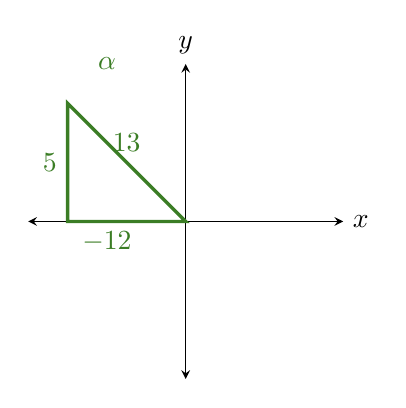
\begin{tikzpicture}
    \draw[<->] (-2,0) -- (2,0) node [right] {$x$};
    \draw[<->] (0,-2) -- (0,2) node [above] {$y$};
    \node at (-1,2) [color=OliveGreen] {$\alpha$};
    \draw[very thick, color=OliveGreen] (0,0) -- node [midway, above] {$13$} (-1.5,1.5) -- node [midway, left] {$5$} (-1.5,0) -- cycle;
    \onslide<5->{\node at (-1,0) [below, color=OliveGreen] {$-12$};}
\end{tikzpicture}}
\end{minipage}
\hspace{0.5cm}
\begin{minipage}{0.4\textwidth}
\begin{align*}
    \onslide<3->{x^2 + 5^2 &= 13^2}   \\
    \onslide<4->{x &= -12}
\end{align*}
\end{minipage}
\end{frame}

\begin{frame}{Example 4}
\begin{minipage}{0.5\textwidth}
\begin{tikzpicture}
    \draw[<->] (-2,0) -- (2,0) node [right] {$x$};
    \draw[<->] (0,-2) -- (0,2) node [above] {$y$};
    \node at (-1,2) [color=blue] {$\beta$};
    \draw[very thick, color=blue] (0,0) -- node [midway, above] {$-1$} (-1.5,0) -- node [midway, left] {$-2$} (-1.5,-1.5) -- cycle;
    \onslide<4->{\node at (-1,-1) [xshift=0.25cm, color=blue] {$\sqrt{5}$};}
\end{tikzpicture}
\end{minipage}
\hspace{0.5cm}
\begin{minipage}{0.4\textwidth}
\begin{align*}
    \onslide<2->{1^2 + 2^2 &= r^2}   \\
    \onslide<3->{r &= \sqrt{5}}
\end{align*}
\end{minipage}
\end{frame}


\begin{frame}[c]{Example 4}
\begin{center}
\setlength{\extrarowheight}{6pt}
    \begin{tabular}{cc}
        ${\color{OliveGreen}\alpha}$ & ${\color{blue}\beta}$    \\ \hline
        $x = -12$   &   $x = -1$    \\
        $y = 5$     &   $y = -2$    \\
        $r = 13$    &   $r = \sqrt{5}$  
    \end{tabular}
\end{center}
\end{frame}

\begin{frame}{Example 4 \quad \scriptsize $x_\alpha = -12, y_\alpha = 5, r_\alpha = 13$ \quad $x_\beta = -1, y_\beta = -2, r_\beta = \sqrt{5}$}
(a) \quad   $\sin(\alpha - \beta)$
\begin{align*}
    \onslide<2->{\sin(\alpha - \beta) &= (\sin\alpha)(\cos\beta) - (\sin\beta)(\cos\alpha)} \\[6pt]
    \onslide<3->{&= \left(\frac{5}{13}\right)\left(\frac{-1}{\sqrt{5}}\right)-\left(\frac{-2}{\sqrt{5}}\right)\left(\frac{-12}{13}\right)}   \\[6pt]
    \onslide<4->{&= \left(\frac{5}{13}\right)\left(\frac{-\sqrt{5}}{5}\right)-\left(\frac{-2\sqrt{5}}{5}\right)\left(\frac{-12}{13}\right)}    \\[6pt]
    \onslide<5->{&= \frac{-5\sqrt{5}}{65} - \frac{24\sqrt{5}}{65}}  \\[6pt]
    \onslide<6->{&= \frac{-29\sqrt{5}}{65}}
\end{align*}
\end{frame}


\begin{frame}{Example 4 \quad \scriptsize $x_\alpha = -12, y_\alpha = 5, r_\alpha = 13$ \quad $x_\beta = -1, y_\beta = -2, r_\beta = \sqrt{5}$}
(b) \quad   $\sin(\alpha + \beta)$
\begin{align*}
    \onslide<2->{\sin(\alpha+\beta) &= -\frac{5\sqrt{5}}{65} + \frac{24\sqrt{5}}{65}} \\[8pt]
    \onslide<3->{&= \frac{19\sqrt{5}}{65}}
\end{align*}
\end{frame}


\begin{frame}{Example 4 \quad \scriptsize $x_\alpha = -12, y_\alpha = 5, r_\alpha = 13$ \quad $x_\beta = -1, y_\beta = -2, r_\beta = \sqrt{5}$}
(c) \quad   $\cos(\alpha - \beta)$
\begin{align*}
    \onslide<2->{\cos(\alpha - \beta) &= (\cos\alpha)(\cos\beta) + (\sin\alpha)(\sin\beta)} \\[6pt]
    \onslide<3->{&= \left(\frac{-12}{13}\right)\left(\frac{-\sqrt{5}}{5}\right)+\left(\frac{5}{13}\right)\left(\frac{-2\sqrt{5}}{5}\right)}   \\[6pt]
    \onslide<4->{&= \frac{12\sqrt{5}}{65} + \frac{-10\sqrt{5}}{65}}  \\[6pt]
    \onslide<6->{&= \frac{2\sqrt{5}}{65}}
\end{align*}
\end{frame}


\begin{frame}{Example 4 \quad \scriptsize $x_\alpha = -12, y_\alpha = 5, r_\alpha = 13$ \quad $x_\beta = -1, y_\beta = -2, r_\beta = \sqrt{5}$}
(d) \quad   $\cos(\alpha + \beta)$
\begin{align*}
    \onslide<2->{\cos(\alpha + \beta) &= \frac{12\sqrt{5}}{65} - \frac{-10\sqrt{5}}{65}} \\[6pt]
    \onslide<3->{&= \frac{22\sqrt{5}}{65}}   
\end{align*}
\end{frame}


\begin{frame}{Example 4 \quad \scriptsize $x_\alpha = -12, y_\alpha = 5, r_\alpha = 13$ \quad $x_\beta = -1, y_\beta = -2, r_\beta = \sqrt{5}$}
(e) \quad   $\tan(\alpha - \beta)$
\begin{align*}
    \onslide<2->{\tan(\alpha - \beta) &= \frac{\tan\alpha - \tan\beta}{1+(\tan\alpha)(\tan\beta)}} \\[6pt]
    \onslide<3->{&= \frac{\frac{-5}{12}-2}{1+\left(\frac{-5}{12}\right)(2)}} \\[6pt]
    \onslide<4->{&= \frac{\frac{-29}{12}}{\frac{2}{12}}} \onslide<5->{\left(\frac{12}{12}\right)} \\[6pt]
    \onslide<6->{&= \frac{-29}{2}}
\end{align*}
\end{frame}

\begin{frame}{Example 4 \quad \scriptsize $x_\alpha = -12, y_\alpha = 5, r_\alpha = 13$ \quad $x_\beta = -1, y_\beta = -2, r_\beta = \sqrt{5}$}
(e) \quad   $\tan(\alpha - \beta)$
\begin{align*}
    \onslide<2->{\tan(\alpha - \beta) &= \frac{\sin(\alpha-\beta)}{\cos(\alpha - \beta)}} \\[6pt]
    \onslide<3->{&= \frac{ \frac{-29\sqrt{5}}{65} }{ \frac{2\sqrt{5}}{65} }} \onslide<4->{\left(\frac{65}{65}\right)} \\[6pt]
    \onslide<5->{&=\frac{-29\sqrt{5}}{2\sqrt{5}}} \\[6pt]
    \onslide<6->{&= \frac{-29}{2}}
\end{align*}
\end{frame}

\end{document}


